\documentclass{standalone}
\usepackage{tikz}
\usetikzlibrary{patterns, positioning}

\begin{document}
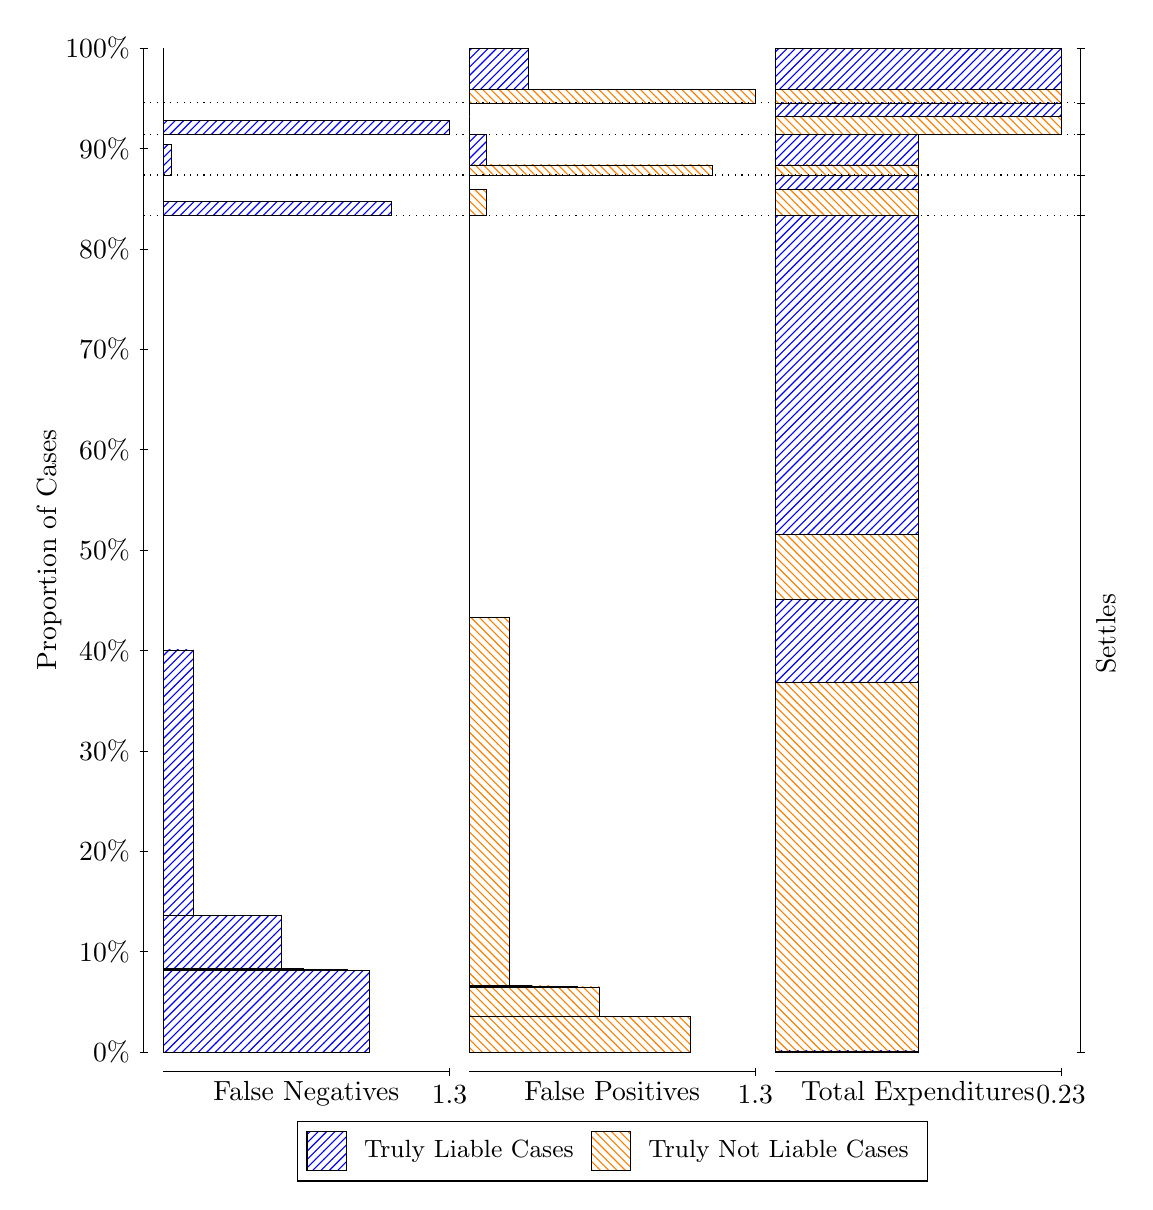
\begin{tikzpicture}
\draw[black, very thin] (1.5,1.75) -- (1.5,14.5);
\node[rotate=90, anchor=center] at (0.3, 8.125) {Proportion of Cases};
\draw[black, very thin] (1.45,1.75) -- (1.55,1.75);
\node[anchor=east] at (1.45, 1.75) {0\%};
\draw[black, very thin] (1.45,3.025) -- (1.55,3.025);
\node[anchor=east] at (1.45, 3.025) {10\%};
\draw[black, very thin] (1.45,4.3) -- (1.55,4.3);
\node[anchor=east] at (1.45, 4.3) {20\%};
\draw[black, very thin] (1.45,5.575) -- (1.55,5.575);
\node[anchor=east] at (1.45, 5.575) {30\%};
\draw[black, very thin] (1.45,6.85) -- (1.55,6.85);
\node[anchor=east] at (1.45, 6.85) {40\%};
\draw[black, very thin] (1.45,8.125) -- (1.55,8.125);
\node[anchor=east] at (1.45, 8.125) {50\%};
\draw[black, very thin] (1.45,9.4) -- (1.55,9.4);
\node[anchor=east] at (1.45, 9.4) {60\%};
\draw[black, very thin] (1.45,10.675) -- (1.55,10.675);
\node[anchor=east] at (1.45, 10.675) {70\%};
\draw[black, very thin] (1.45,11.95) -- (1.55,11.95);
\node[anchor=east] at (1.45, 11.95) {80\%};
\draw[black, very thin] (1.45,13.225) -- (1.55,13.225);
\node[anchor=east] at (1.45, 13.225) {90\%};
\draw[black, very thin] (1.45,14.5) -- (1.55,14.5);
\node[anchor=east] at (1.45, 14.5) {100\%};

\draw[black, very thin] (13.4,1.75) -- (13.4,14.5);
\draw[black, very thin] (13.35,1.75) -- (13.45,1.75);
\node[anchor=west] at (13.35, 1.75) {};
\draw[black, very thin] (13.35,12.371) -- (13.45,12.371);
\node[anchor=west] at (13.35, 12.371) {};
\draw[black, very thin] (13.35,12.887) -- (13.45,12.887);
\node[anchor=west] at (13.35, 12.887) {};
\draw[black, very thin] (13.35,13.406) -- (13.45,13.406);
\node[anchor=west] at (13.35, 13.406) {};
\draw[black, very thin] (13.35,13.804) -- (13.45,13.804);
\node[anchor=west] at (13.35, 13.804) {};
\draw[black, very thin] (13.35,14.5) -- (13.45,14.5);
\node[anchor=west] at (13.35, 14.5) {};

\draw[black, very thin, pattern color=blue, pattern=north east lines] (1.75,1.75) rectangle (4.3702,2.7865);
\draw[black, very thin, pattern color=blue, pattern=north east lines] (1.75,2.7865) rectangle (4.0907,2.7948);
\draw[black, very thin, pattern color=blue, pattern=north east lines] (1.75,2.7948) rectangle (3.8112,2.8035);
\draw[black, very thin, pattern color=blue, pattern=north east lines] (1.75,2.8035) rectangle (3.5317,2.813);
\draw[black, very thin, pattern color=blue, pattern=north east lines] (1.75,2.813) rectangle (3.2522,3.4854);
\draw[black, very thin, pattern color=blue, pattern=north east lines] (1.75,3.4854) rectangle (2.1343,6.8558);
\draw[black, very thin, pattern color=orange, pattern=north west lines] (1.75,6.8558) rectangle (1.75,12.371);
\draw[black, very thin, pattern color=blue, pattern=north east lines] (1.75,12.371) rectangle (4.6497,12.554);
\draw[black, very thin, pattern color=orange, pattern=north west lines] (1.75,12.554) rectangle (1.75,12.887);
\draw[black, very thin, pattern color=blue, pattern=north east lines] (1.75,12.887) rectangle (1.8548,13.278);
\draw[black, very thin, pattern color=orange, pattern=north west lines] (1.75,13.278) rectangle (1.75,13.406);
\draw[black, very thin, pattern color=blue, pattern=north east lines] (1.75,13.406) rectangle (5.3833,13.579);
\draw[black, very thin, pattern color=orange, pattern=north west lines] (1.75,13.579) rectangle (1.75,13.804);
\draw[black, very thin, pattern color=orange, pattern=north west lines] (1.75,13.804) rectangle (1.75,13.978);
\draw[black, very thin, pattern color=blue, pattern=north east lines] (1.75,13.978) rectangle (1.75,14.5);
\draw[black, very thin, pattern color=orange, pattern=north west lines] (5.6333,1.75) rectangle (8.4393,2.1978);
\draw[black, very thin, pattern color=orange, pattern=north west lines] (5.6333,2.1978) rectangle (7.2881,2.5756);
\draw[black, very thin, pattern color=orange, pattern=north west lines] (5.6333,2.5756) rectangle (7.0003,2.5826);
\draw[black, very thin, pattern color=orange, pattern=north west lines] (5.6333,2.5826) rectangle (6.7125,2.5891);
\draw[black, very thin, pattern color=orange, pattern=north west lines] (5.6333,2.5891) rectangle (6.4248,2.5952);
\draw[black, very thin, pattern color=orange, pattern=north west lines] (5.6333,2.5952) rectangle (6.137,7.2647);
\draw[black, very thin, pattern color=blue, pattern=north east lines] (5.6333,7.2647) rectangle (5.6333,12.371);
\draw[black, very thin, pattern color=orange, pattern=north west lines] (5.6333,12.371) rectangle (5.8492,12.704);
\draw[black, very thin, pattern color=blue, pattern=north east lines] (5.6333,12.704) rectangle (5.6333,12.887);
\draw[black, very thin, pattern color=orange, pattern=north west lines] (5.6333,12.887) rectangle (8.7271,13.015);
\draw[black, very thin, pattern color=blue, pattern=north east lines] (5.6333,13.015) rectangle (5.8492,13.406);
\draw[black, very thin, pattern color=orange, pattern=north west lines] (5.6333,13.406) rectangle (5.6333,13.631);
\draw[black, very thin, pattern color=blue, pattern=north east lines] (5.6333,13.631) rectangle (5.6333,13.804);
\draw[black, very thin, pattern color=orange, pattern=north west lines] (5.6333,13.804) rectangle (9.2667,13.978);
\draw[black, very thin, pattern color=blue, pattern=north east lines] (5.6333,13.978) rectangle (6.3888,14.5);
\draw[black, very thin, pattern color=orange, pattern=north west lines] (9.5167,1.75) rectangle (11.333,1.7561);
\draw[black, very thin, pattern color=blue, pattern=north east lines] (9.5167,1.7561) rectangle (11.333,1.7643);
\draw[black, very thin, pattern color=orange, pattern=north west lines] (9.5167,1.7643) rectangle (11.333,6.4473);
\draw[black, very thin, pattern color=blue, pattern=north east lines] (9.5167,6.4473) rectangle (11.333,7.5021);
\draw[black, very thin, pattern color=orange, pattern=north west lines] (9.5167,7.5021) rectangle (11.333,8.3277);
\draw[black, very thin, pattern color=blue, pattern=north east lines] (9.5167,8.3277) rectangle (11.333,12.371);
\draw[black, very thin, pattern color=orange, pattern=north west lines] (9.5167,12.371) rectangle (11.333,12.704);
\draw[black, very thin, pattern color=blue, pattern=north east lines] (9.5167,12.704) rectangle (11.333,12.887);
\draw[black, very thin, pattern color=orange, pattern=north west lines] (9.5167,12.887) rectangle (11.333,13.015);
\draw[black, very thin, pattern color=blue, pattern=north east lines] (9.5167,13.015) rectangle (11.333,13.406);
\draw[black, very thin, pattern color=orange, pattern=north west lines] (9.5167,13.406) rectangle (13.15,13.631);
\draw[black, very thin, pattern color=blue, pattern=north east lines] (9.5167,13.631) rectangle (13.15,13.804);
\draw[black, very thin, pattern color=orange, pattern=north west lines] (9.5167,13.804) rectangle (13.15,13.978);
\draw[black, very thin, pattern color=blue, pattern=north east lines] (9.5167,13.978) rectangle (13.15,14.5);
\draw[black, dotted] (1.5,12.371) -- (13.4,12.371);
\draw[black, dotted] (1.5,12.887) -- (13.4,12.887);
\draw[black, dotted] (1.5,13.406) -- (13.4,13.406);
\draw[black, dotted] (1.5,13.804) -- (13.4,13.804);
\draw[black, very thin] (1.75,1.5) -- (5.3833,1.5);
\node[anchor=north] at (3.5667, 1.5) {False Negatives};
\draw[black, very thin] (5.3833,1.45) -- (5.3833,1.55);
\node[anchor=north] at (5.3833, 1.45) {1.3};

\draw[black, very thin] (5.6333,1.5) -- (9.2667,1.5);
\node[anchor=north] at (7.45, 1.5) {False Positives};
\draw[black, very thin] (9.2667,1.45) -- (9.2667,1.55);
\node[anchor=north] at (9.2667, 1.45) {1.3};

\draw[black, very thin] (9.5167,1.5) -- (13.15,1.5);
\node[anchor=north] at (11.333, 1.5) {Total Expenditures};
\draw[black, very thin] (13.15,1.45) -- (13.15,1.55);
\node[anchor=north] at (13.15, 1.45) {0.23};

\node[black, centered, rotate=90] at (13.72, 7.0603) {Settles};





\draw (7.449999999999999,1.5) node[draw=none] (baseCoordinate) {};
\begin{scope}[align=center]
        \matrix[scale=0.5, draw=black, below=0.5cm of baseCoordinate, nodes={draw}, column sep=0.1cm]{
            \node[rectangle, draw, minimum width=0.5cm, minimum height=0.5cm, pattern=north east lines, pattern color=blue] {}; &
            \node[draw=none, font=\small] (B) {Truly Liable Cases}; &
            \node[rectangle, draw, minimum width=0.5cm, minimum height=0.5cm, pattern=north west lines, pattern color=orange] {}; &
            \node[draw=none, font=\small] (B) {Truly Not Liable Cases}; \\
            };
\end{scope}

\end{tikzpicture}
\end{document}